\section{}
% The system shown, represents a floor of mass 𝑀 supported by springs of stiffness 𝑘. A mass 𝑚 is 
% % dropped on the floor from a height of ℎ.
% a) (5 pts) Determine the motion of the floor using 𝑥, the displacement from the static 
% equilibrium configuration before impact.
% b) (5 pts) Determine the maximum displacement for the case when ℎ = 0. NOTE: Do not 
% neglect the weight of the floor and the weight of mass 𝑚

The system shown, represents a floor of mass $M$ supported by springs of stiffness $k$. A mass $m$ is
dropped on the floor from a height of $h$.
\begin{figure}[h]
    \centering
    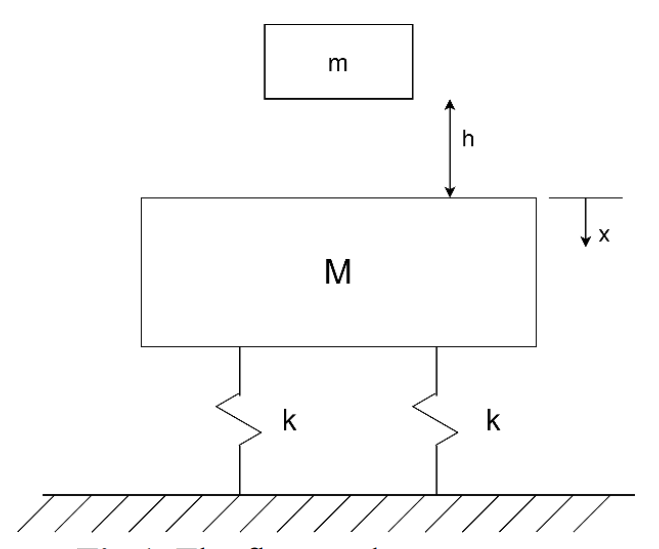
\includegraphics[width=0.5\linewidth]{Questions/Figures/q5 problem diagram.png}
    \caption{The floor and mass system}
    \label{fig:q5-png}
\end{figure}
\begin{enumerate}[label=(\alph*)]
    \item (5 pts) Determine the motion of the floor using $x$, the displacement from the static
        equilibrium configuration before impact.
    \item (5 pts) Determine the maximum displacement for the case when $h = 0$. NOTE: Do not
        neglect the weight of the floor and the weight of mass $m$
\end{enumerate}

\subsection*{Solution}
\subsection{}
First define
\begin{itemize}
    \item State 1 is the initial state of $m$ at rest at height $h$.
    \item State 2 is the state of $m$ just before impact at height $h = 0$.
    \item State 3 is the state of $m$ just after impact with $M$.
\end{itemize}
and assume
\begin{itemize}
    \item The collision is perfectly inelastic.
    \item $m$ is dropped with no initial velocity.
    \item $M$ is initially at rest.
    \item The springs are initially at their equilibrium length.
\end{itemize}
We begin the analysis by considering Work-Energy Theorem on mass $m$ initially and just before impact:
\begin{align*}
    T_1 + U_{1 \to 2} &= T_2 \\
    \implies 0 + m g h &= \frac{1}{2} m v_2^2 \\
    \implies v_2 &= \sqrt{2 g h}
\end{align*}
Next, we employ Conservation of Momentum on the system of $m$ and $M$ before and after impact. 
\begin{align*}
    m v_2 &= (m + M) v_3 \\
    \implies v_3 &= \frac{m}{m + M} v_2 \\
    \implies v_3 &= \frac{m}{m + M} \sqrt{2 g h}
\end{align*}
This gives us the initial velocity of the oscillator with $m_{\text{eff}} = m + M$. Next, we must determine the effect of $m$ on the equilibrium position.
\begin{figure}[h]
    \centering
    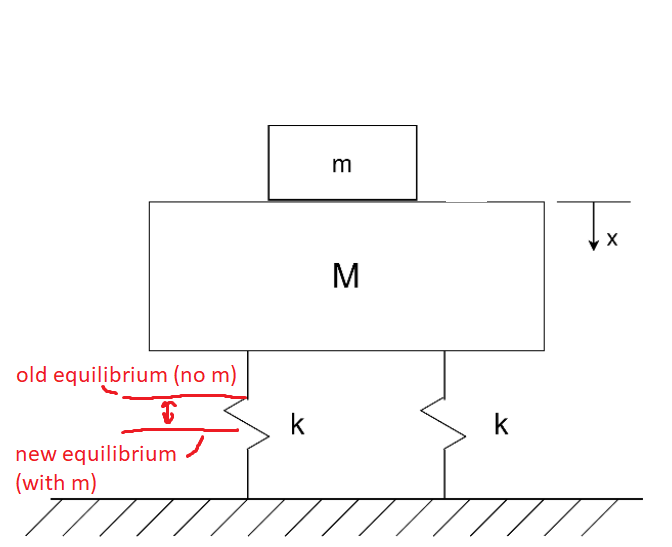
\includegraphics[width=0.5\linewidth]{Questions/Figures/q5 equilibrium change.png}
    \caption{The equilibrium position of the oscillator}
    \label{fig:q5_equilibrium_change-png}
\end{figure}
The equilibrium position of the oscillator can be found using Hooke's Law. Since the springs are in parallel, the effective stiffness is the sum of the individual stiffnesses.
\begin{align*}
    F &= k_{\text{eff}} \delta_{st} \\
    \implies \delta_{st} &= \frac{mg}{k_{\text{eff}}} \\
    &= \frac{mg}{2k}
\end{align*}
Since $x$ is defined as positive sense downwards, the initial conditions are:
\begin{align*}
    x(0) &= -\frac{mg}{2k} \\
    \dot{x}(0) &= \frac{m}{m + M} \sqrt{2 g h}
\end{align*}
Note that the negative sign on $x(0)$ is because the new equilibrium position is below the original equilibrium position. Now we define the natural frequency of this system:
\begin{align*}
    \Aboxed{p = \sqrt{\frac{k_{\text{eff}}}{m_{\text{eff}}}} = \sqrt{\frac{2k}{m + M}}}
\end{align*}
From (eq. 2.7), 
\begin{align*}
    x(t) &= x_0 \cos (pt) + \frac{\dot{x}_0}{p} \sin (pt) \\
    \Aboxed{x(t) &= -\frac{mg}{2k} \cos (pt) + \frac{m\sqrt{2gh}}{p(m + M)} \sin (pt)}
\end{align*}

\subsection{}
Using the single-term form of the response, 
\begin{gather*}
    x(t) = X \sin (pt + \phi) \\
    X = \sqrt{x_0^2 + \left(\frac{\dot{x}_0}{p}\right)^2} \\
    \phi = \tan^{-1} \left(\frac{x_0}{\dot{x}_0 / p}\right)
\end{gather*}
So the maximum displacement is the amplitude, $X$, which is
\begin{align*}
    \Aboxed{x_{\text{max}} &= \sqrt{\left(-\frac{mg}{2k}\right)^2 + \left(\frac{m\sqrt{2gh}}{p(m + M)}\right)^2}}
\end{align*}
%asd